\documentclass{standalone}


\usepackage{tikz}
\usetikzlibrary{shapes, arrows}
\usetikzlibrary{arrows,calc,decorations.markings,math,arrows.meta}
\usetikzlibrary{positioning}
% \usepackage{xcolor}
\usepackage{graphicx}




\begin{document}
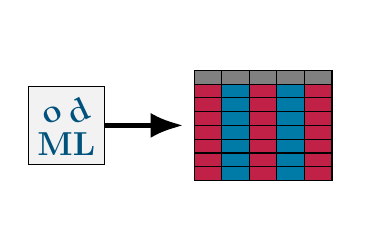
\begin{tikzpicture}
		    \definecolor{col1}{rgb}{0.76, 0.13, 0.28}
		    \definecolor{col2}{rgb}{0.0, 0.48, 0.65}
		    \definecolor{odmlcolor}{rgb}{0.00,0.32,0.49}
		    \definecolor{back}{rgb}{0.95,0.95,0.95}
		    \node(odml) [draw,align=center,font=\bfseries,fill=back]{\large \textcolor{odmlcolor}{\rotatebox[origin=c]{25}{o}\rotatebox[origin=c]{25}{d}} \\ \large{\textcolor{odmlcolor}{ML}}};
		    \node[right = 1cm of odml] (table) {\tikz{
		    \begin{scope}[scale=0.7]
		      \foreach \x in {-0.75,...,1.5}{
			  \draw[xstep=2,col1,line width=10] (\x,-1) -- (\x,1);
			  }
		      \foreach \x in {-0.25,...,1.5}{
			  \draw[xstep=2,col2,line width=10] (\x,-1) -- (\x,1);
			  }
		    \end{scope}
		    \fill [gray,scale=.35] (-2,1.5) rectangle (3,2);
		    \begin{scope}[scale=0.35]
		      \draw[xstep=1,ystep=0.5] (-2,-2) grid (3,2);
		    \end{scope}
		    }};
		    
		    \node[above = 0cm of table](tabletext) {};
		    
		    \draw[-{Latex[scale=1]},line width=0.7mm] (odml.east) -- (table.west) {};
\end{tikzpicture}
\end{document}